% -*- latex -*-
%%%%%%%%%%%%%%%%%%%%%%%%%%%%%%%%%%%%%%%%%%%%%%%%%%%%%%%%%%%%%%%%
%%%%%%%%%%%%%%%%%%%%%%%%%%%%%%%%%%%%%%%%%%%%%%%%%%%%%%%%%%%%%%%%
%%%%
%%%% This text file is part of the source of 
%%%% `Parallel Computing'
%%%% by Victor Eijkhout, copyright 2012/3
%%%%
%%%%%%%%%%%%%%%%%%%%%%%%%%%%%%%%%%%%%%%%%%%%%%%%%%%%%%%%%%%%%%%%
%%%%%%%%%%%%%%%%%%%%%%%%%%%%%%%%%%%%%%%%%%%%%%%%%%%%%%%%%%%%%%%%

\Level 0 {Basics}

\Level 1 {The OpenMP model}

OpenMP is based on on two concepts: the use of of \indexterm{threads}
and the \indextermdef{fork/join model} of
parallelism. For now you can think of a thread as a sort of process:
the computer executes a sequence of instructions.
The fork/join model says that a thread can split itself (`fork')
into a number of threads that are identical copies. At some point
these copies go away and the original thread is left (`join'),
but while the \indextermsub{team of}{threads} exists,
you have parallelism available to you. The part of the execution
between fork and join is known as a \indexterm{parallel region}.

Figure~\ref{fig:forkjoin} gives a simple picture of this:
a thread forks into a team of threads, and these threads
themselves can fork again.
\begin{figure}[ht]
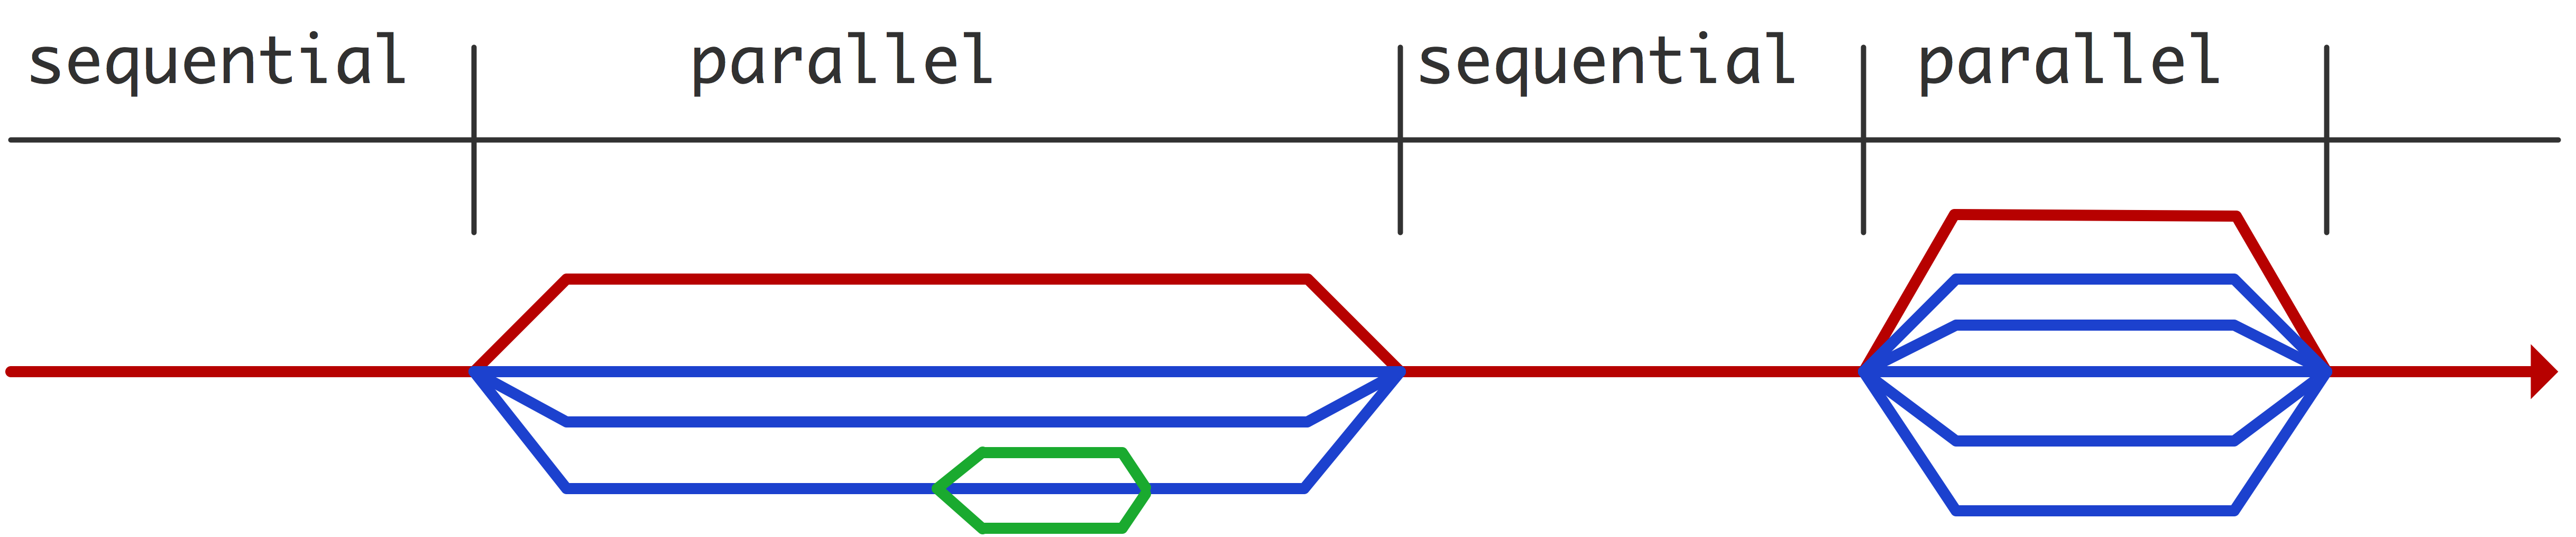
\includegraphics[scale=.08]{fork-join}
\caption{Thread creation and deletion during parallel execution}
\label{fig:forkjoin}
\end{figure}

The threads that are forked are all copies of the
\emph{master thread}\index{threads!master}: they have access to all that was
computed so far; this is their \indexterm{shared data}.  Of course, if
the threads were completely identical the parallelism would be
pointless, so they also have private data, and they can identify
themselves: they know their thread number.  This allows you to do
meaningful parallel computations with threads.

This brings us to the third important concept: that of \indexterm{work sharing}
constructs. In a team of threads, initially there will be replicated execution;
a work sharing construct divides available parallelism over the threads.

So there you have it: OpenMP uses teams of threads, and inside
a parallel region the work is distributed over the threads with a work sharing construct.
Threads can access shared data, and they have some private data.

For more on threads, see \HPSCref{sec:threads}.

\Level 1 {OpenMP language constructs}

Of course, OpenMP is not magic, so you have to tell it when something
can be done in parallel. This is mostly done through \indexterm{directives},
and to a lesser extent through library calls.

The first thing we want to do is create a parallel region.
Here is a very simple example:
\verbatimsnippet{hello-omp}
or in Fortran
\verbatimsnippet{hello-omp-f}
It prints out the `hello world' message once for each thread. How many
threads there are can be determined in a number of ways; we will get to that later.

This code corresponds to the model we just discussed:
\begin{itemize}
\item Immediately preceding the parallel block, one thread will be
  executing the code. In the main program this is the \emph{initial
    thread}\index{threads!initial}.
\item At the start of the block, a new \indextermsub{team of}{threads} is
  created, and the thread that was active before the block
  becomes the \emph{master thread}\index{threads!master} of that team.
\item Each thread in the team then executes the body of the block; it
  will have access to all variables of the surrounding environment.
\end{itemize}

\Level 1 {Directives}
\commandref{omp-directives}

Directives look like \indextermsub{cpp}{directives}, but they
are actually handled by the compiler, not the preprocessor.
In C/C++, a~directive is followed by a single command or a block
in curly braces; in Fortran there is a matching end directive
for every opening directive.

\Level 2 {Parallel regions}
\commandref{omp-parallel}

The simplest way to create a parallel region is through the 
\indexpragma{parallel} pragma. In~C this is followed by a block,
in Fortran you conclude the block with \texttt{end parallel}.
\begin{verbatim}
#pragma omp parallel
{
  // this is executed by all threads
}
\end{verbatim}
It would be pointless to have the block be executed identically by
all threads, so you will probably use the function
\indextermtt{omp_get_thread_num}, to find out which thread you are,
and execute work that is individual to that thread.
There is also a function
\indextermtt{omp_get_num_threads} to find out the total number of threads.
Both these functions give a number relative to the current team;
recall from figure~\ref{fig:forkjoin} that new teams can be created recursively.

\begin{exercise}
  Take the `hello world' program above, and modify it so that you get
  multiple messages to you screen, saying
\begin{verbatim}
  Hello from thread 0 out of 4!
  Hello from thread 2 out of 4!
\end{verbatim}
  and so on. What happens if you set your number of threads larger than the available
  cores on your computer?
\end{exercise}

\begin{exercise}
  What happens if you call \n{omp_get_thread_num} and \n{omp_get_num_threads}
  outside a parallel region?
\end{exercise}

\begin{exercise}
  Test nested parallelism. First of all, set \n{OMP_NESTED} to
  \n{TRUE}. Now write an OpenMP program as follows:
  \begin{enumerate}
  \item Write a subprogram that contains a parallel region.
  \item Write a main program with a parallel region; call the subprogram both inside and outside the parallel region.
    \item Insert print statements 
      \begin{enumerate}
      \item in the main program outside the parallel region,
      \item in the parallel region in the main program,
      \item in the subprogram outside the parallel region,
      \item in the parallel region inside the subprogram.
      \end{enumerate}
  \end{enumerate}
  Run your program and count how many print statements of each type you get.
\end{exercise}

\Level 2 {Thread data}

A thread has access to variables of two kinds. Variables on the
\indexterm{heap} are typically created by a call to \indextermtt{malloc}
(in~C) or \indextermtt{new} (in~C++). Threads that are spawned have
the same type of access to them.

There are also variables on the \indexterm{stack}, which have a local
\indexterm{scope}. Thread access to such variables is more complicated,
since each thread has its own \indexterm{context}. Most relevant to our story,
the context can contain local copies of variables, that is, each thread
has a variable, say~\n{x}, but they are local to each thread context.
Thus, one thread setting the value of its instance of~\n{x} has no influence on what
another thread sees as the value of its instance of~\n{x}.

To use the technical term, there are
\begin{itemize}
\item \indexterm{shared variables},
  where each thread refers to the same data item, and 
\item \indexterm{private variables},
  where each thread has its own instance.
\end{itemize}
%
\begin{figure}[ht]
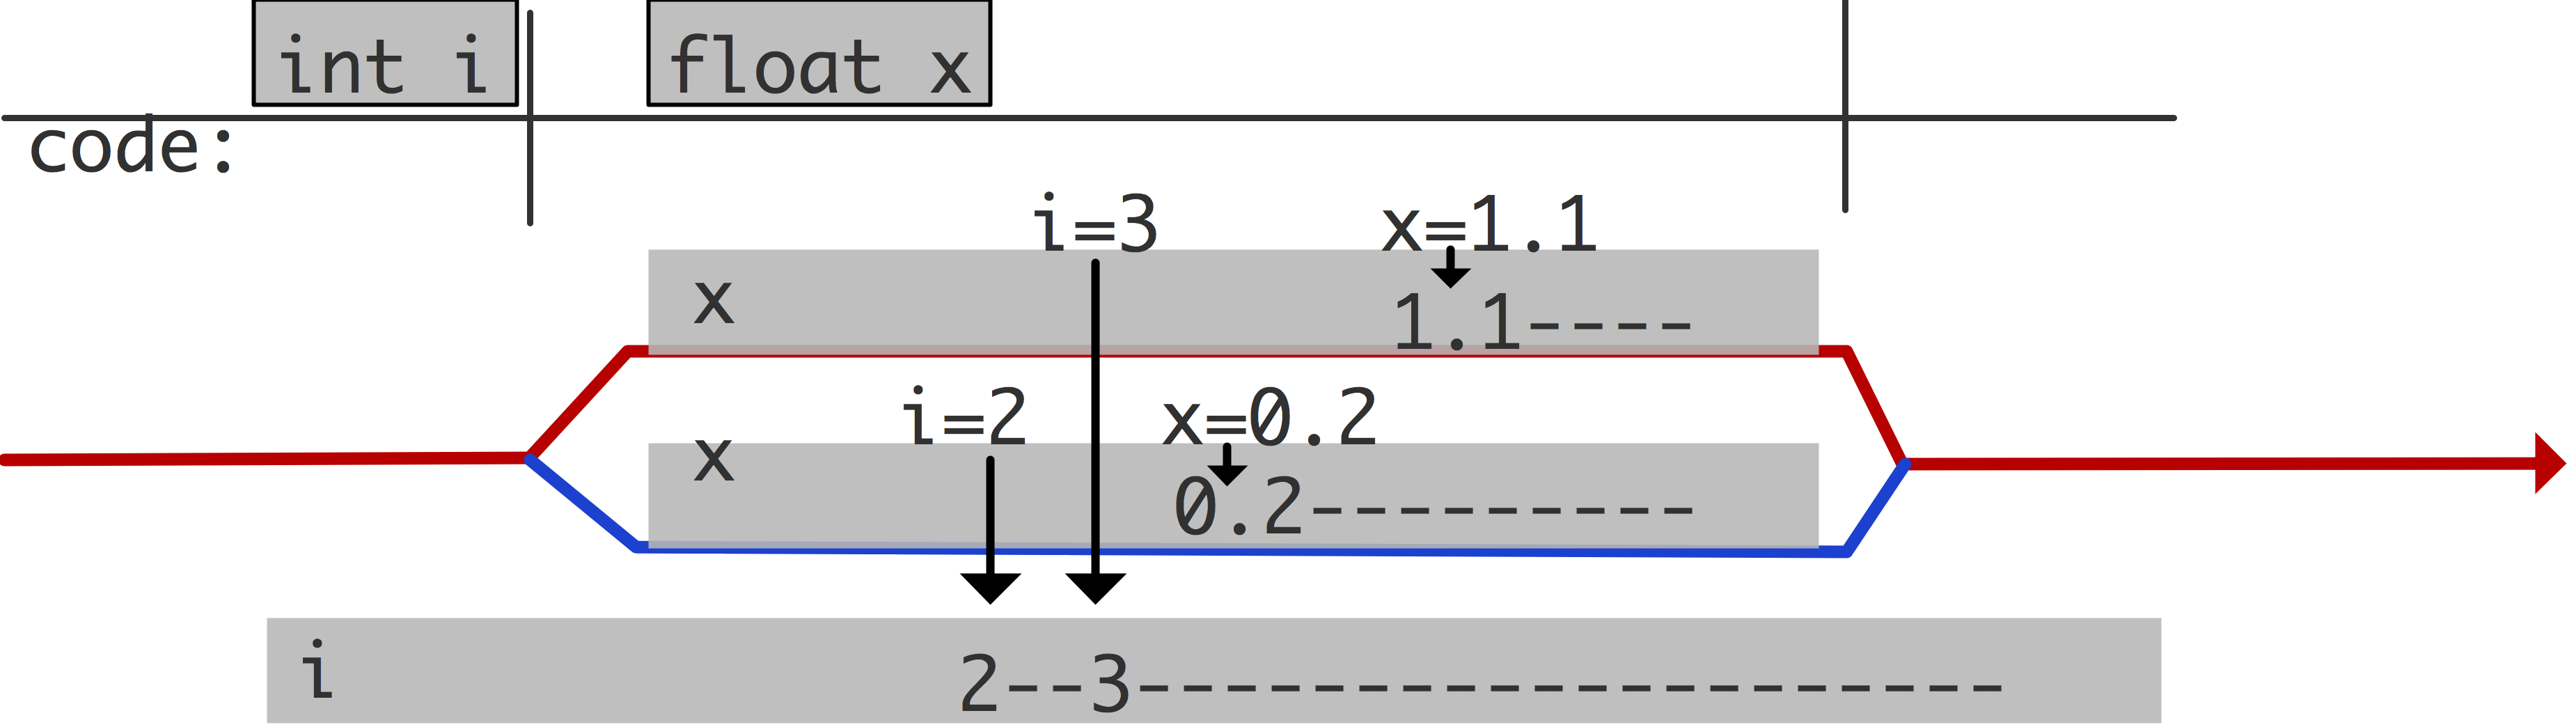
\includegraphics[scale=.1]{fork-join-vars}
\caption{Locality of variables in threads}
\label{fig:threadvars}
\end{figure}
%
This is illustrated in figure~\ref{fig:threadvars}.

When a new \emph{thread team}\index{thread!team!and variable access} is created,
there are various mechanisms for indicating which variables are shared
and which are private.
\begin{itemize}
\item By default, any variable declared in the surrounding scope is
  shared. Thus, in the following code segment, each thread sets the
  value of~\n{x}, and its value after the parallel region is
  indeterminate because you do not know in what sequence the threads
  performed the update.
\begin{verbatim}
int x;
#omp parallel
{
  x = omp_get_thread_num();
}
// what is the value of x?
\end{verbatim}
\item Any variable declared inside the parallel region is private. In
  the following code segment the variable~\n{x} is local to the
  thread: the value that is set by one thread does not interfere with
  what other threads do.
\begin{verbatim}
#omp parallel
{
  double x;
  x = // some dynamic value
  ... = .... x ....
}
\end{verbatim}
  Since the parallel region is also a \indexterm{lexical scope}, the
  variable~\n{x} does not exist after the parallel region. (In Fortran
  this mechanism of local allocation does not exist, so this question
  does not come up.)
\item In a parallel loop, the loop variable is private, even though it may
  have been declared outside the parallel construct.
\item A variable declared in the surrounding scope can explicitly be
  declared private or shared by adding a \indexpragma{private}
  or \indexpragma{shared} clause respectively to the OpenMP
  directive. In the following fragment, each 
  For the behaviour of shared variables, the default, see the point above.
\item Unless otherwise stated, private variables are undefined at the
  start of the parallel region, and disappear at the end; shared
  variables become undefined after the parallel region.
\item Data allocated on the \indexterm{heap} is
  shared\footnote{However, note that the C~and~Fortran standards do
    not actually define a~heap. Therefore it is wise to spell out your
    intentions.}.
\end{itemize}

\Level 1 {OpenMP code structure}
\commandref{omp-code-structure}

OpenMP is largely based on directives: instructions to the compiler
and runtime that are hidden in comment-like structures. In Fortran,
the directives are actually in a comment:
\begin{verbatim}
!$OMP construct
\end{verbatim}
while in C they are hidden in a \indexterm{pragma}: something that
is normally meant for the \indextermbus{C}{preprocessor}:
\begin{verbatim}
#pragma omp construct
\end{verbatim}
After the directive, in~C you usually find a `structured block':
a single statement or a block in curly braces. In~Fortran,
the directive is explicitly closed with
\begin{verbatim}
!$OMP END construct
\end{verbatim}

Above, you saw the \indexpragma{parallel} directive: when a thread
encounters it, it spawns new threads to form a \indextermbus{thread}{team}.
This team stays active during the execution of the \indexterm{structured block}
that follows, after which only the master thread remains. However,
in addition to this lexical description of thread activity, the thread team
also stays intact in any code that is dynamically encountered. For instance,
any subroutines called the OpenMP \indexterm{construct} are also executed
in parallel.

\Level 1 {Some externalities}

\Level 2 {Compiling}

Your file or Fortran module needs to contain
\begin{verbatim}
#include "omp.h"
\end{verbatim}
in C, and 
\begin{verbatim}
use omp_lib
\end{verbatim}
for Fortran.

OpenMP is handled by extensions to your regular compiler, typically by
adding an option to your commandline:
\begin{verbatim}
# gcc
gcc -o foo foo.c -fopenmp
# Intel compiler
icc -o foo foo.c -openmp
\end{verbatim}
If you have separate compile and link stages, you need that option in both.

When you use the openmp compiler option, a \indexterm{cpp} variable \indextermtt{_OPENMP}
will be defined. Thus, you can have conditional compilation by writing
\begin{verbatim}
#ifdef _OPENMP
   ...
#else
   ...
#endif
\end{verbatim}

\Level 2 {Running an OpenMP program}

You run an OpenMP program by invoking it the regular way (for instance \n{./a.out}),
but its behaviour is influenced by some \indextermbus{OpenMP}{environment variables}.
The most important one is \indextermtt{OMP_NUM_THREADS}:
\begin{verbatim}
export OMP_NUM_THREADS=8
\end{verbatim}
which sets the number of threads that a program will use.
See section~\ref{ref:omp-environ} for a list of all environment variables.

\Level 0 {Creating parallelism}

The \indexterm{fork/join model} of OpenMP means that you need some way of
indicating where an activity can be forked for independent execution.
There are two ways of doing this:
\begin{enumerate}
\item You can declare a parallel region and
  split one thread into a whole team of threads. We will discuss this next
  in section~\ref{sec:parallelregion}. The division of the work over the threads
  is controlled by \indexterm{work sharing construct} (section~\ref{sec:work-sharing}).
\item Alternatively, you can use tasks and indicating one parallel
  activity at a time. You will see this in section~\ref{sec:omp:task}.
\end{enumerate}

Note that OpenMP only indicates how much parallelism is present;
whether independent activities are in fact executed in parallel
is a runtime decision. The factors influencing this are discussed
in section~\ref{sec:omp-howmany}.

\Level 1 {Parallel regions}
\commandref{parallelregion}

The simplest way to create parallelism in OpenMP is to use
the \indexpragma{parallel} pragma. A~block preceded by the \n{omp parallel} pragma
is executed by a newly created team of threads. 
This is an instance of the \indexac{SPMD} model: all threads execute the same
segment of code.
Since it would not be interesting to have all threads do the same calculations,
you can use the function \indexcommand{omp_get_thread_num} to distinguish 
between them.

For instance, if you program computes
\begin{verbatim}
result = f(x)+g(x)+h(x)
\end{verbatim}
you could parallelize this as
\begin{verbatim}
double result = 0;
#pragma omp parallel
{
  int num = omp_get_thread_num();
  if (num==0)      result += f(x);
  else if (num==1) result += g(x);
  else if (num==2) result += h(x);
}
\end{verbatim}
This example shows how the three functions are computed in parallel,
but other than that \textbf{there are many things wrong with this example}.
The rest of this section will be about explaining what is wrong here,
and what can be done about it.

\Level 1 {Just how many threads?}
\commandref{omp-howmany}

Declaring a parallel region tells OpenMP that a team of threads can be created.
The actual size of the team depends on various factors (see section~\ref{ref:omp-environ}
for variables and functions mentioned in this section).
\begin{itemize}
\item The \emph{environment variable}\index{OpenMP!environment
  variables} \indextermtt{OMP_NUM_THREADS} limits the number of
  threads that can be created.
\item If you don't set this variable, you can also set this limit
  dynamically with the \emph{library routine}\index{OpenMP!library
    routines} \indextermtt{omp_set_num_threads}. This routine takes
  precedence over the aforementioned environment variable if both are
  specified.
\item A limit on the number of threads can also be set as a clause
  on a parallel region.
\end{itemize}
If you specify a greater amount of parallelism than the hardware supports,
the runtime system will probably ignore your specification and choose a lower value.
To ask how much parallelism is actually used in your parallel region,
use \indextermtt{omp_get_num_threads}. To query these hardware limits,
use \indextermtt{omp_get_num_procs}.

Another limit on the number of threads is imposed when you use nested parallel regions.
This can arise if you have a parallel region in a subprogram which is sometimes called
sequentially, sometimes in parallel. The variable \indextermtt{OMP_NESTED} controls
whether the inner region will create a team of more than one thread.

\Level 1 {Thread data in parallel regions}

OpenMP is a programming system for shared memory. This means that
you often want all threads to see the same data; we call this `shared' data.
However, sometimes you want a thread to have `private' data, for instance
for intermediate results in a computation.

Private variables act as if they are created at the start of the parallel region.
If a variable by that name already exists in the surrounding scope,
that variable will become inaccessible. Here is a clear example of a private variable,
created inside the parallel region:
\begin{verbatim}
int x = 5;
#pragma omp parallel
{ 
  int x = 6;
}
// x is still 5
\end{verbatim}
This example is pretty much the same:
\begin{verbatim}
int x = 5;
#pragma omp parallel private(x)
{ 
  x = 6;
}
// x is still 5
\end{verbatim}
We will discuss all this in detail in section~\ref{sec:ompdata}.

\Level 0 {Work sharing}
\commandref{work-sharing}

The declaration of a \indexterm{parallel region} establishes a team of
threads. This offers the possibility of parallelism, but to actually
get meaningful parallel activity you need something more.
OpenMP uses the concept of a \indexterm{work sharing
construct}: a way of dividing parallelizable work over a team of threads.
The work sharing constructs are:
\begin{itemize}
\item \texttt{for/do} The threads divide up the loop iterations among
  themselves; see~\ref{sec:omp-for}.
\item \texttt{sections} The threads divide a fixed number of sections
  between themselves; see section~\ref{sec:omp-sections}.
\item \texttt{single} The section is executed by a single thread; section~\ref{sec:omp-single}.
\item \texttt{task}
\item \texttt{workshare} Can parallelize Fortran array syntax.
\end{itemize}

\Level 1 {Loop parallelism}
\commandref{omp-for}

The parallel execution of a loop can be handled a number of different ways.
For instance, you can create a parallel region around the loop, and
adjust the loop bounds:
\begin{verbatim}
#pragma omp parallel
{
  int threadnum = omp_get_thread_num(),
    numthreads = omp_get_num_threads();
  int low = N*threadnum/numthreads,
    high = N*(threadnum+1)/numthreads;
  for (i=low; i<high; i++)
    // do something with i
}
\end{verbatim}

A more natural option is to use the
\indexpragma{parallel for} pragma:
\begin{verbatim}
#pragma omp parallel
#pragma omp for
for (i=0; i<N; i++) {
  // do something with i
}
\end{verbatim}
This has several advantages. For one, you don't have to calculate the loop bounds
for the threads yourself, but you can also tell OpenMP to assign the loop
iterations according to different schedules (section~\ref{sec:schedule}).

Figure~\ref{fig:omp-par-do} shows the execution on four threads of
\begin{verbatim}
#pragma omp parallel
{
  code1();
#pragma omp for
  for (i=1; i<=4*N; i++) {
    code2();
  }
  code3();
}
\end{verbatim}
The code before and after the loop is executed identically
in each thread; the loop iterations are spread over the four threads.
\begin{figure}[ht]
  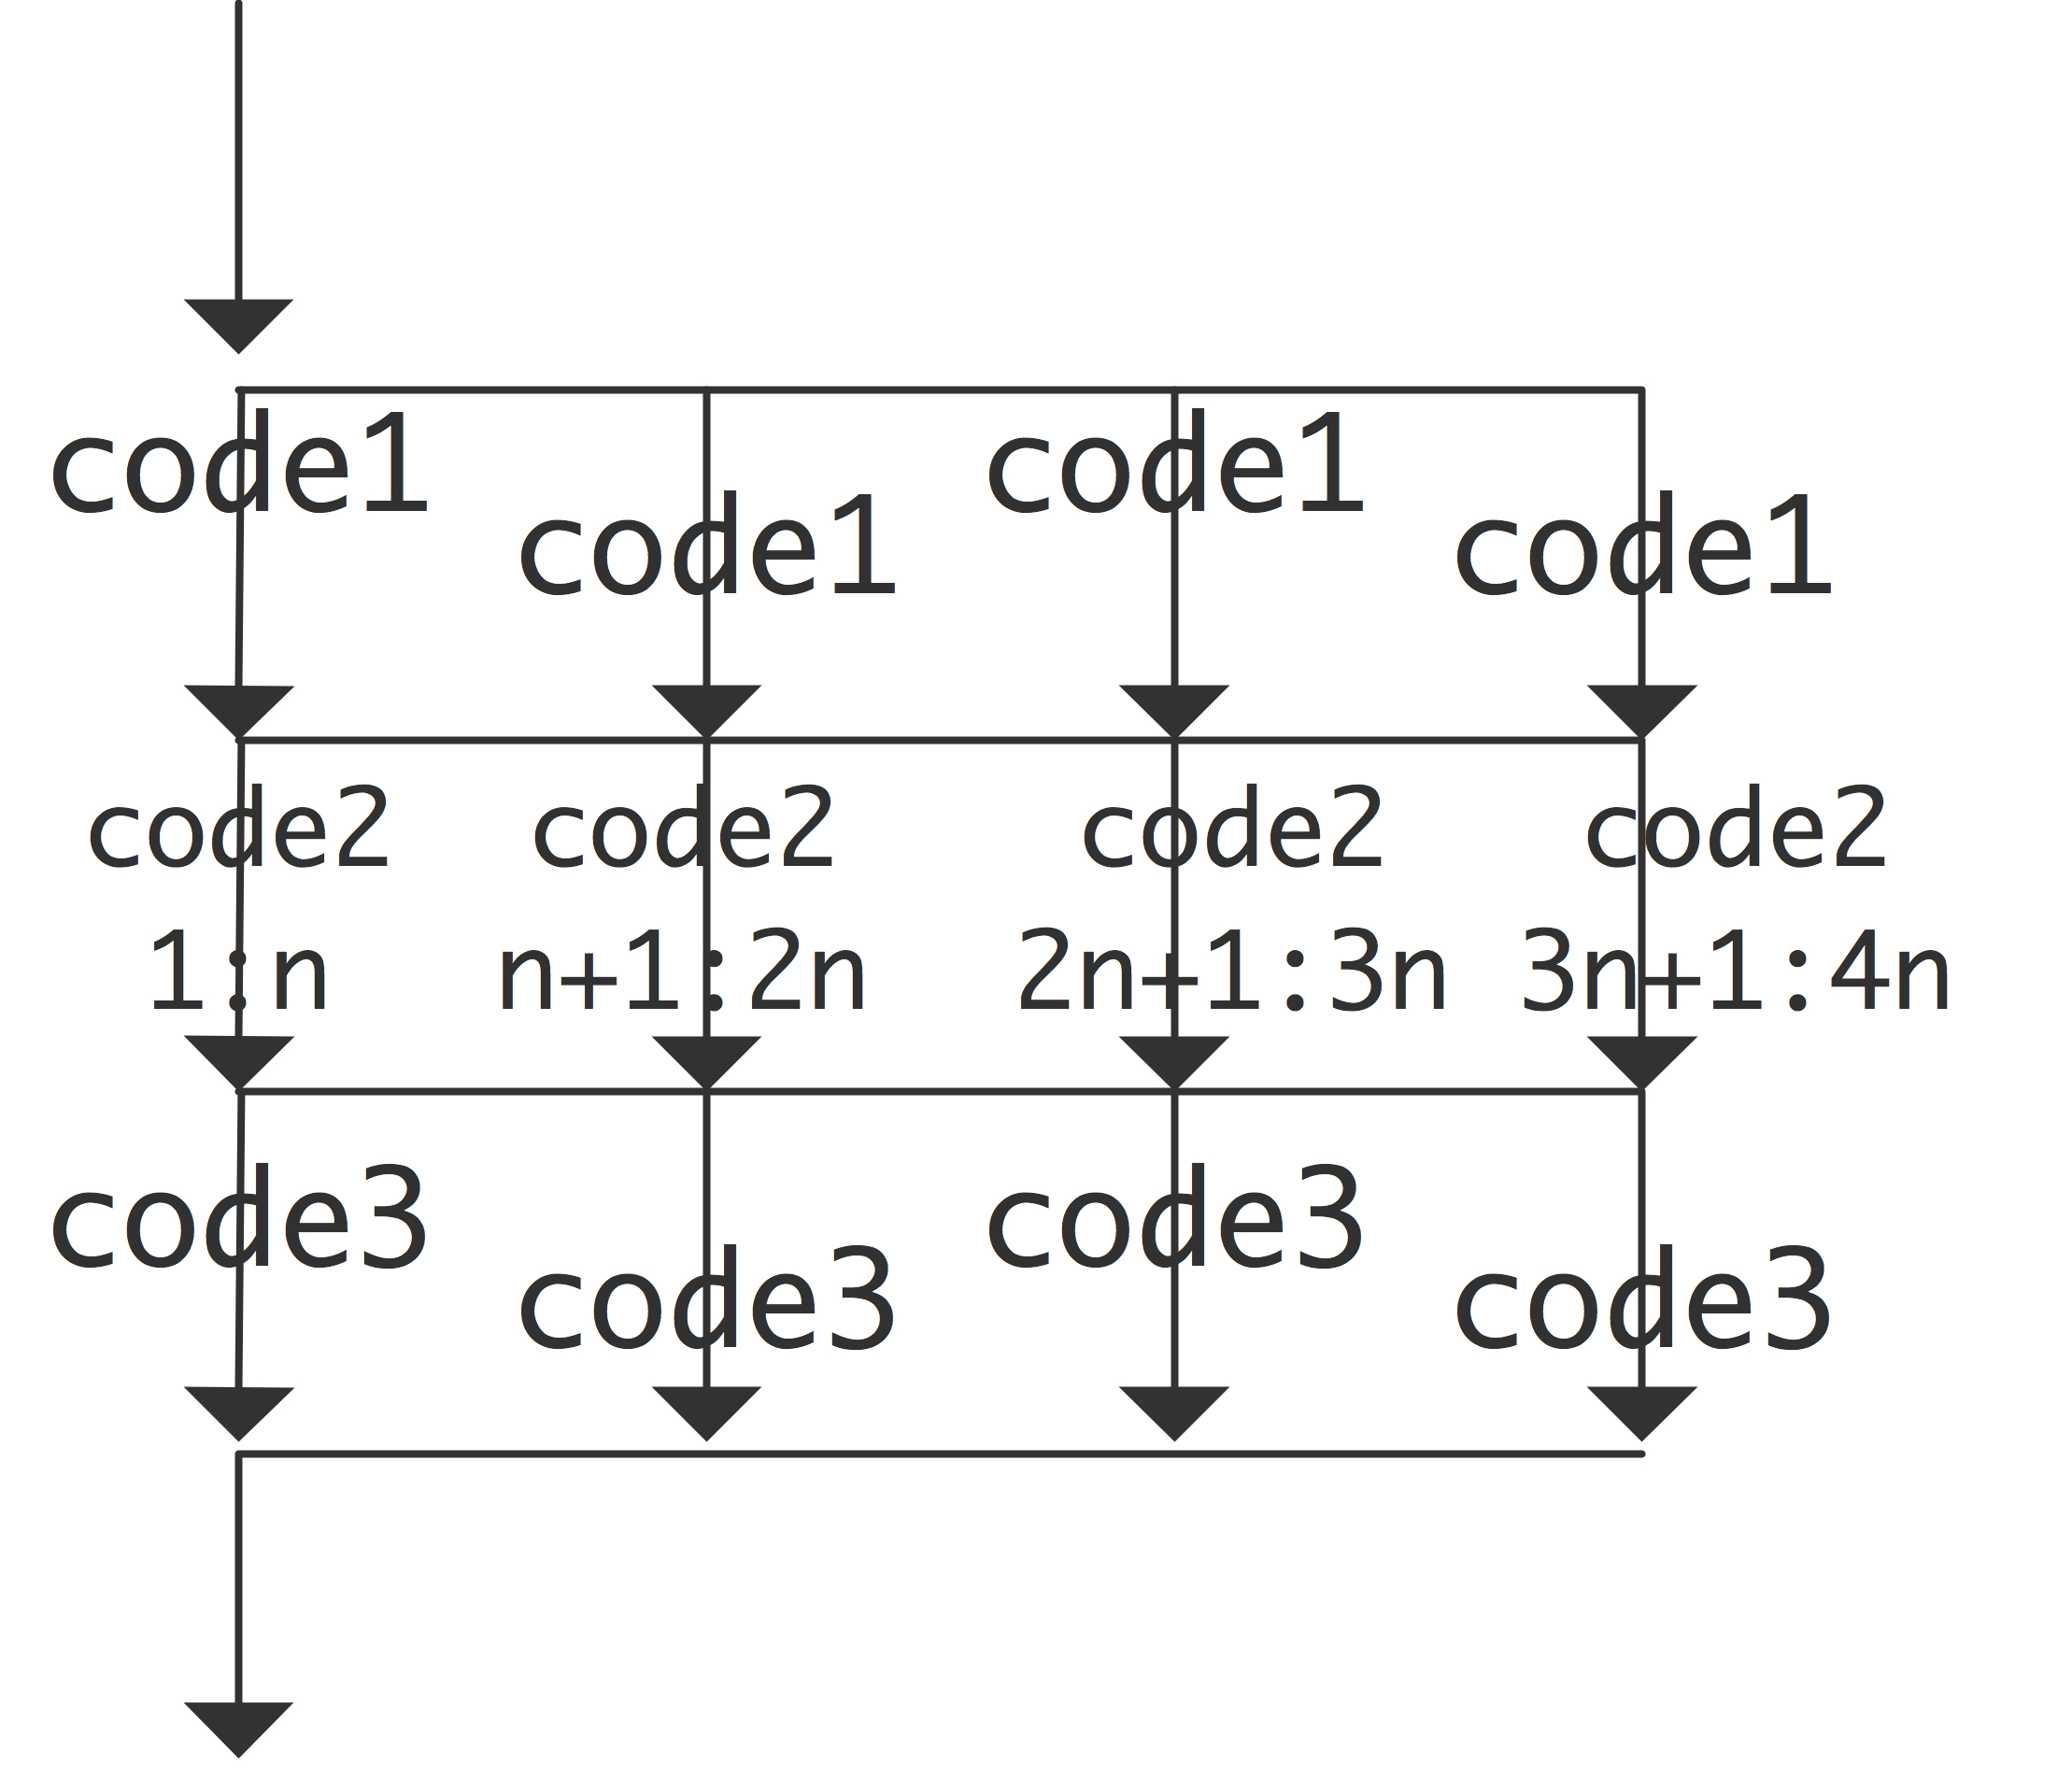
\includegraphics[scale=.1]{parallel-do}
  \caption{Execution of parallel code inside and outside a loop}
  \label{fig:omp-par-do}
\end{figure}

Instead of having two pragmas, one for the parallel region and one for
worksharing over the loop iterations, you can combine the two:
\begin{verbatim}
#pragma omp parallel for
  for (i=0; .....
\end{verbatim}

The loop has to satisfy a number of basic constraints, such as that you can not
jump out of it.

\Level 2 {Loop schedules}
\commandref{sec:schedule}

Usually you will have many more iterations in a loop than there are threads.
Thus, there are several ways you can assign your loop iterations to the threads.
OpenMP lets you specify this with the \indextermtt{schedule} clause.
\begin{verbatim}
#pragma omp for schedule(....)
\end{verbatim}

The first distinction we now have to make is between static and dynamic schedules.
With static schedules, the iterations are assigned purely based on the number
of iterations and the number of threads (and the \n{chunk} parameter; see later).
In dynamic schedules, on the other hand, iterations are assigned to threads that
are unoccupied. Dynamic schedules are a good idea if iterations take an unpredictable
amount of time, so that \indexterm{load balancing} is needed.

\begin{figure}[ht]
  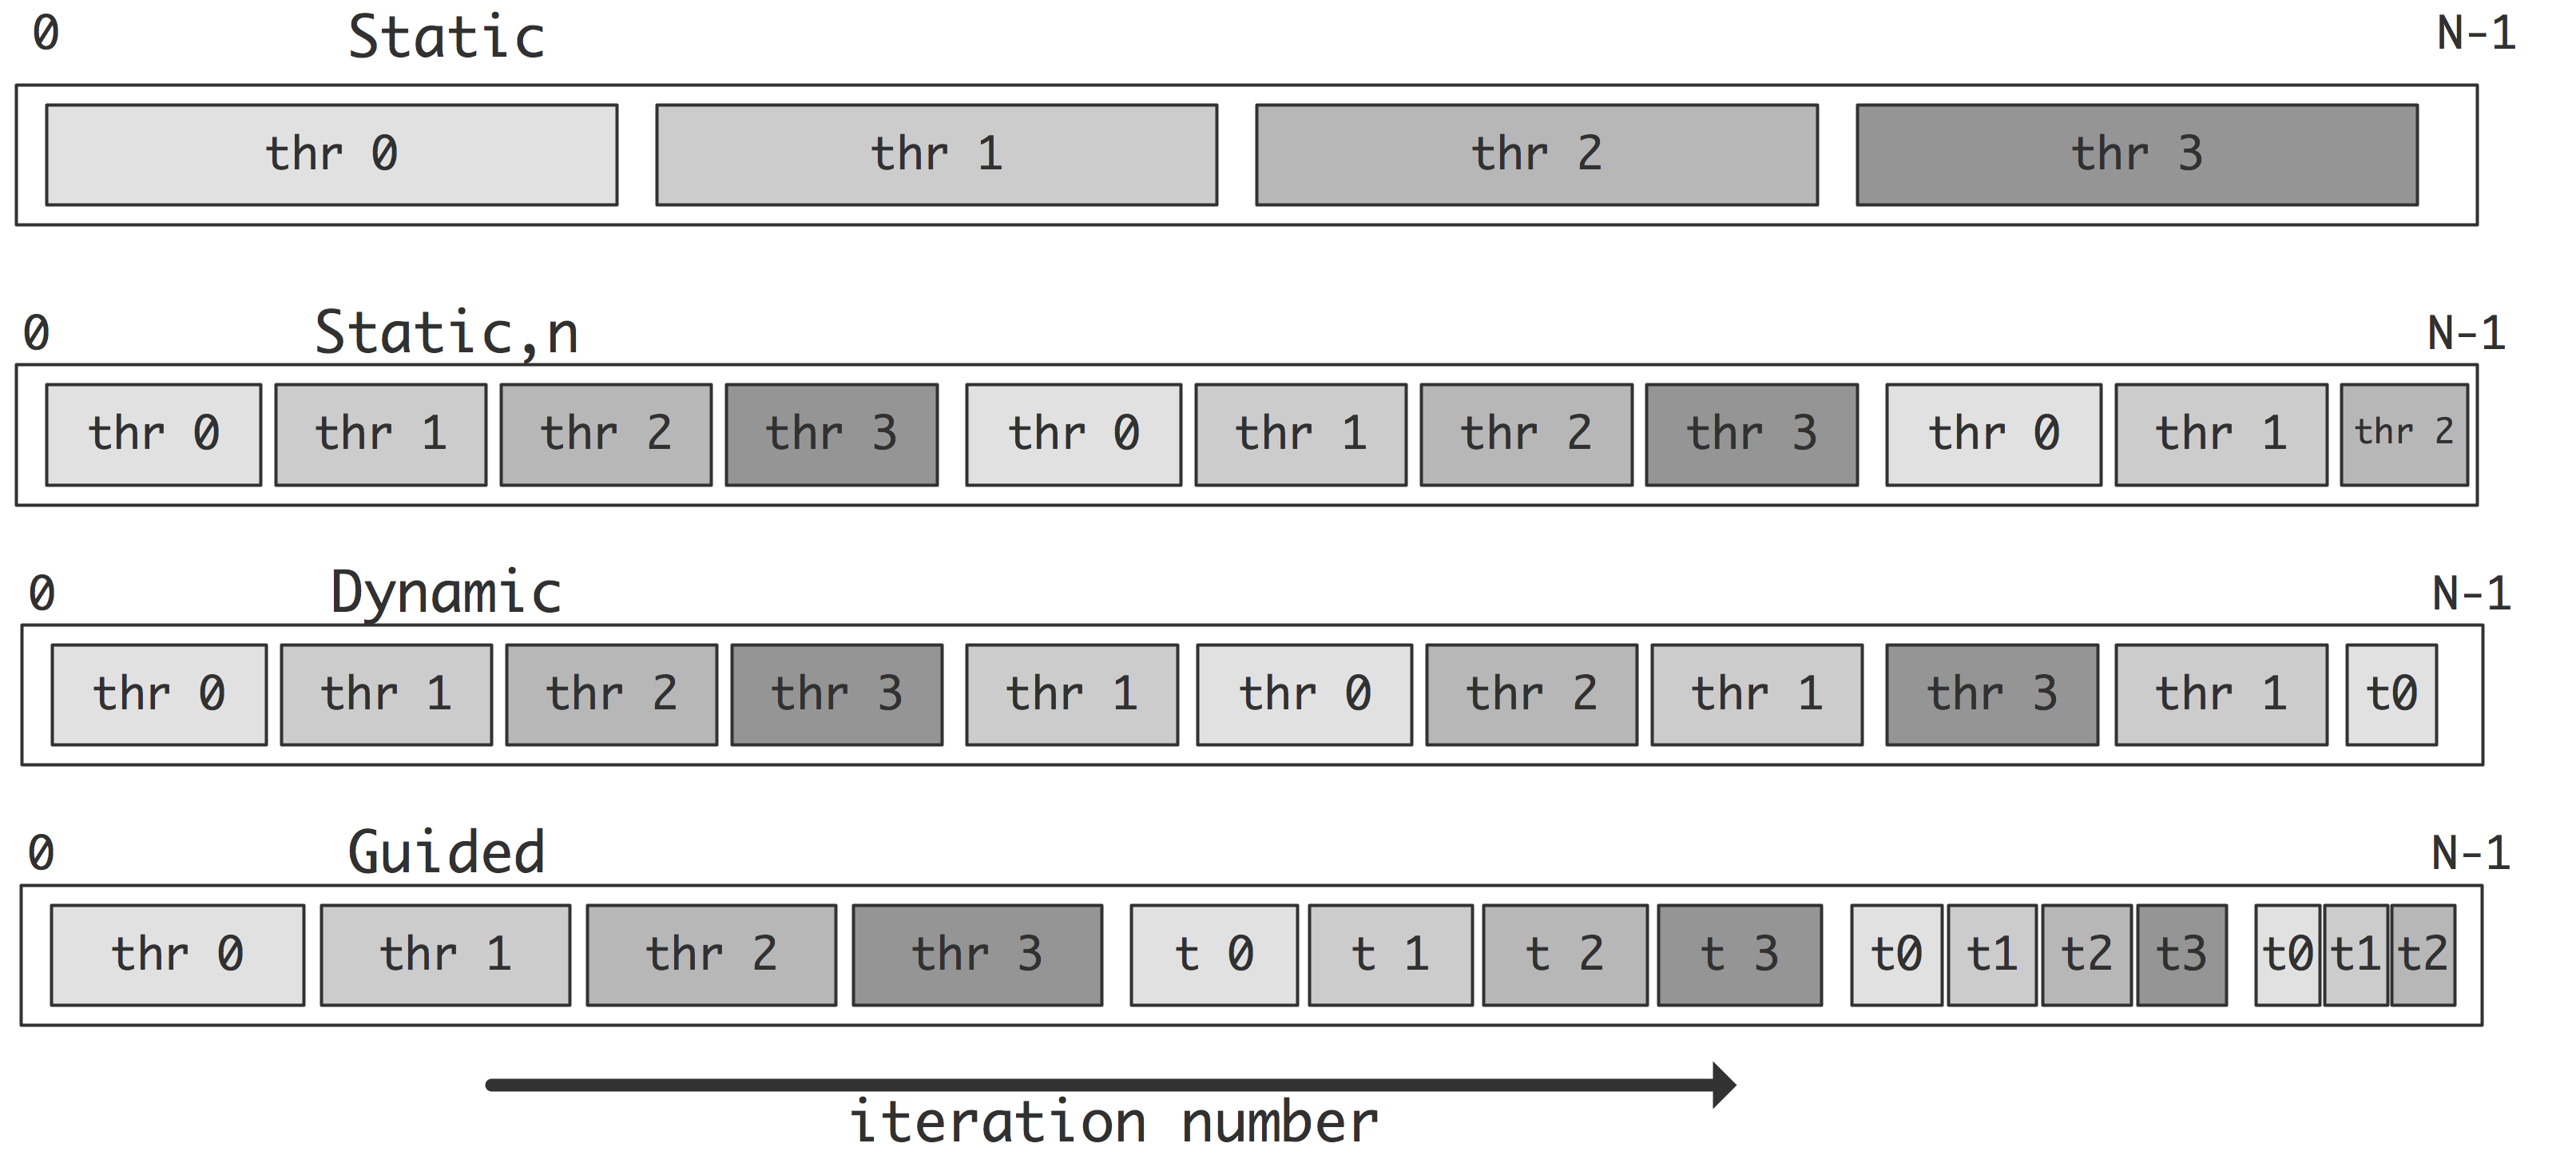
\includegraphics[scale=.12]{schedules}
  \caption{Illustration of the loop scheduling strategies}
  \label{fig:omp-schedule}
\end{figure}

The default static schedule is to assign one consecutive block of iterations
to each thread. If you want different sized blocks you can defined a \indexclauseoption{schedule}{chunk} size:
\begin{verbatim}
#omp pragma for schedule(static[,chunk])
\end{verbatim}
(where the square brackets indicate an optional argument).
With static scheduling, the compiler will split up the loop iterations at compile time,
so, provided the iterations take roughly the same amount of time, this is the most efficient at runtime.

The choice of a chunk size is often a balance between the low overhead of having 
only a few chunks, versus the load balancing effect of having smaller chunks.
\begin{exercise}
  Why is a chunk size of~1 typically a bad idea? (Hint: think about
  cache lines, and read \HPSCref{sec:falseshare}.)
\end{exercise}

In dynamic scheduling OpenMP will put blocks of iterations
(the default chunk size is~1) in a task queue, and the threads take one of these
tasks whenever they are finished with the previous.
\begin{verbatim}
#omp pragma for schedule(static[,chunk])
\end{verbatim}
While this schedule may give good load balancing if the iterations
take very differing amounts of time to execute, it does carry runtime
overhead for managing the queue of iteration tasks.

Finally, there is the \indexclauseoption{schedule}{guided} schedule, which gradually decreases the chunk size.
The thinking here is that large chunks carry the least overhead, but smaller chunks are better
for load balancing.
%
The various schedules are illustrated in figure~\ref{fig:omp-schedule}.

If you don't want to decide on a schedule in your code, you can
specify the \indexclauseoption{schedule}{runtime} schedule. The actual
schedule will then at runtime be read from the
\indextermtt{OMP_SCHEDULE} environment variable. You can even just
leave it to the runtime library by specifying
\indexclauseoption{schedule}{auto}

\begin{exercise}
  Program the \indexterm{LU factorization} algorithm without pivoting.
\begin{verbatim}
for k=1,n:
  A[k,k] = 1./A[k,k]
  for i=k+1,n:
    A[i,k] = A[i,k]/A[k,k]
    for j=k+1,n:
      A[i,j] = A[i,j] - A[i,k]*A[k,j]
\end{verbatim}
\begin{enumerate}
\item Argue that it is not possible to parallelize the outer loop.
\item Argue that it is possible to parallelize both the $i$ and $j$ loops.
\item Parallelize the algorithm by focusing on the $i$ loop. Why is the algorithm as given here best
  for a matrix on row-storage? What would you do if the matrix was on column storage?
\item Argue that with the default schedule, if a row is updated by one thread in one iteration,
  it may very well be updated by another thread in another. Can you find a way to schedule
  loop iterations so that this does not happen? What practical reason is there for doing so?
\end{enumerate}
\end{exercise}

\Level 2 {Reductions}

There is an extended discussion of reductions in section~\ref{sec:reduction}

\Level 2 {\texttt{nowait}}

The implicit barrier at the end of a work sharing construct
can be cancelled with a \indexclause{nowait} clause.
This has the effect that threads that are finished can continue
with the next code in the parallel region:
\begin{verbatim}
#pragma omp parallel
{
#pragma omp for nowait
  for (i=0; i<N; i++) { ... }
  // more parallel code
}
\end{verbatim}

In the following example, threads that are finished with the first loop
can start on the second. Note that this requires both loops to have
the same schedule.
\begin{verbatim}
#pragma omp parallel
{
  x = local_computation()
#pragma omp for nowait
  for (i=0; i<N; i++) { 
    x[i] = ... 
  }
#pragma omp for 
  for (i=0; i<N; i++) { 
    y[i] = ... x[i] ...
  }
}
\end{verbatim}

\Level 2 {While loops}

OpenMP can only handle `for' loops: \indexterm{while loops} can not
be parallelized. So you have to find a way around that. While loops
are for instance used to search through data:
\begin{verbatim}
while ( a[i]!=0 && i<imax ) {
 i++; }
// now i is the first index for which \n{a[i]} is zero.
\end{verbatim}
We replace the while loop by a for loop that examines all locations:
\begin{verbatim}
result = -1;
#omp parallel for
for (i=0; i<imax; i++) {
  if (a[i]!=0 && result<0) result = i;
}
\end{verbatim}
\begin{exercise}
  Show that this code has a race condition.
\end{exercise}
You can fix the race condition by making the condition into a critical section;
section~\ref{sec:critical}. In this particular example, with a very small amount
of work per iteration, that is likely to be inefficient 
in this case (why?).
A~more efficient solution uses the \indexpragma{lastprivate} pragma:
\begin{verbatim}
result = -1;
#omp parallel for lastprivate(result)
for (i=0; i<imax; i++) {
  if (a[i]!=0) result = i;
}
\end{verbatim}
You have now solved a slightly different problem: the result variable
contains the \emph{last} location where \n{a[i]} is zero.

\Level 1 {Sections}
\commandref{omp-sections}

A parallel loop is an example of independent work units that are numbered.
If you have a pre-determined number of independent work units, 
the \indexpragma{sections} is more appropriate. In a \n{sections} construct
can be any number of \indexpragma{section} constructs. These need to be
independent, and they can be execute by any available thread in the current team,
including having multiple sections done by the same thread.
\begin{verbatim}
#pragma omp sections
{
#pragma omp section
  // one calculation
#pragma omp section
  // another calculation
}
\end{verbatim}

This construct can be used to divide large blocks of independent work.
Suppose that in the following line, both \n{f(x)} and \n{g(x)}
are big calculations:
\begin{verbatim}
  y = f(x) + g(x)
\end{verbatim}
You could then write
\begin{verbatim}
double y1,y2;
#pragma omp sections
{
#pragma omp section
  y1 = f(x)
#pragma omp section
  y2 = g(x)
}
y = y1+y2;
\end{verbatim}
Instead of using two temporaries, you could also use a critical
section; see section~\ref{sec:critical}.  However, the best solution
is have a \n{reduction} clause on the \n{sections} directive:
\begin{verbatim}
  y = f(x) + g(x)
\end{verbatim}
You could then write
\begin{verbatim}
y = 0;
#pragma omp sections reduction(+:y)
{
#pragma omp section
  y += f(x)
#pragma omp section
  y += g(x)
}
\end{verbatim}

\Level 1 {Single/master}
\commandref{omp-single}
\indexpragma{master}
\indexpragma{single}

The \indexpragma{single} and \indexpragma{master} pragma
limit the execution of a block to a single thread. 
This can for instance be used to print tracing information
or doing \emph{I/O}\index{I/O!in OpenMP} operations.
\begin{verbatim}
#pragma omp parallel
{
#pragma omp single
  printf("We are starting this section!\n");
  // parallel stuff
}
\end{verbatim}
Another use of \n{single} is to perform initializations
in a parallel region:
\begin{verbatim}
#pragma omp parallel
{
  int a;
  #pragma omp single
    a = f(); // some computation
  #pragma omp sections
    // various different computations using a
}
\end{verbatim}

The point of the single directive in this last example is that the
computation needs to be done only once, because of the shared memory.
Since it's a work sharing construct there is an \emph{implicit
  barrier}\index{implicit barrier!after single directive} after it,
which guarantees that all threads have the correct value in their
local memory (see section~\ref{sec:omp:flush}.

\begin{exercise}
  What is the difference between this approach and how the same
  computation would be parallelized in MPI?
\end{exercise}

The \texttt{master} directive, also enforces execution
on a single thread, specifically the master thread of the team,
but it does not have the synchronization through the implicit barrier.

\begin{exercise}
  Modify the above code to read:
\begin{verbatim}
#pragma omp parallel
{
  int a;
  #pragma omp master
    a = f(); // some computation
  #pragma omp sections
    // various different computations using a
}
\end{verbatim}
  This code is no longer correct. Explain.
\end{exercise}

\Level 1 {Fortran array syntax parallelization}
\commandref{fortran-workshare}

The \n{parallel do} directive is used to parallelize loops,
and this applies to both C and Fortran. However, Fortran also
has implied loops in its \emph{array syntax}\index{Fortran!array syntax}.
To parallelize array syntax you can use the \indexpragma{workshare}
directive.

\Level 0 {Controlling thread data}
\commandref{ompdata}

In a parallel region there are two types of data: private and shared.
In this sections we will see the various way you can control what category
your data falls under; for private data items we also discuss how their values
relate to shared data.

\Level 1 {Shared data}

In a parallel region, any data declared outside it will be shared:
any thread using a variable~\n{x} will  the same memory location
associated with that variable.

Example:
\begin{verbatim}
  int x = 5;
#pragma omp parallel
  {
    x = x+1;
    printf("shared: x is %d\n",x);
  }
\end{verbatim}
All threads increment the same variable, so after the loop it will
have a value of five plus the number of threads; or maybe less because of the data races
involved.

Sometimes this global update is what you want; in other cases the
variable is intended only for intermediate results in a computation.
In that case 
there are various ways of creating
data that is local to a thread, and therefore invisible to other threads.

\Level 1 {Private data}
\commandref{omp-private}

In the C/C++ language it is possible to declare variables inside
a \indexterm{lexical scope}; roughly: inside curly braces.
This concept extends to OpenMP parallel regions and directives:
any variable declared in a block following an OpenMP directive
will be local to the executing thread.

Example:
\begin{verbatim}
  int x = 5;
#pragma omp parallel
  {
    int x; x = 3;
    printf("local: x is %d\n",x);
  }
\end{verbatim}
After the parallel region, the outer variable~\n{x} will still have the value~\n{5}.

The Fortran language does not have this concept of scope, so you have to use a
\indexclause{private} clause:
\begin{verbatim}
!$OMP parallel private(x)
\end{verbatim}

The \indexpragma{private} directive declares data to have a separate copy 
in the memory of each thread. 
Such private variables are initialized as they would be in a main program.
Any computed value goes away at the end 
of the parallel region. (However, see below.)
Thus, you should not rely on any initial value, or on the value of the outer variable
after the region.

\begin{verbatim}
  int x = 5;
#pragma omp parallel private(x)
  {
    x = x+1; // dangerous
    printf("private: x is %d\n",x);
  }
  printf("after: x is %d\n",x); // also dangerous
\end{verbatim}

Private arrays are tricky.
\begin{itemize}
\item In C, if an array is statically defined, e.g.,
\begin{verbatim}
double a[2][5];
\end{verbatim}
declaring \n{private(a)} will indeed put a copy on in each thread.
Note that this will lead to an explosion in memory use; in fact, for large arrays you
  may experience \indextermbus{stack}{overflow}.
\item Dynamically allocated arrays, e.g.,
\begin{verbatim}
double *a; a = (double*) malloc( some_size );
\end{verbatim}
can not be made private with \n{private(a)}: this only gives each thread 
a private pointer, but these pointers all point to the same memory location.
\end{itemize}

\Level 1 {Default}

As remarked, most data in a parallel section is shared. This default behaviour can be 
controlled by adding a \indexpragma{default} clause:
\begin{verbatim}
#pragma omp parallel default(shared) private(x)
{ ... }
#pragma omp parallel default(private) shared(matrix)
{ ... }
\end{verbatim}
and if you want to play it safe:
\begin{verbatim}
#pragma omp parallel default(none) private(x) shared(matrix)
{ ... }
\end{verbatim}

Setting \n{default(none)} is useful for debugging. If your code
behaves differently in parallel from sequential there is probably a data race.
Specifying the status of every variable is a good way to
debug this.

\Level 1 {First and last private}

You can force initialization with \indexclause{firstprivate}.
\begin{verbatim}
  int t=2;
#pragma omp parallel firstprivate(t)
  {
    t += f( omp_get_thread_num() );
    g(t);
  }
\end{verbatim}
The variable \n{t} behaves like a private variable, except that it is
initialized to the outside value.

It is possible to preserve a private variable
from the last iteration with \indexclause{lastprivate}:
\begin{verbatim}
#pragma omp parallel for \
        lastprivate(tmp)
for (i=0; i<N; i+) {
  tmp = ......
  x[i] = .... tmp ....
}
..... tmp ....
\end{verbatim}

\Level 1 {Persistent data}

Most data in OpenMP parallel regions is either inherited
from the master thread and therefore shared, or temporary within the scope of the
region and fully private.
There is also a mechanism for data that is private to a thread, but not limited
in lifetime to one parallel region.
The \indexpragma{threadprivate} pragma is used to declare that each thread
is to have a private copy of a variable:
\begin{verbatim}
#pragma omp threadprivate(var)
\end{verbatim}
This variable will then have the lifetime of an ordinary variable,
but inside a parallel region the private copy is used.

\Level 0 {Reductions}
\commandref{reduction}

Parallel tasks often produce some quantity that needs to be summed
or otherwise combined.
In section~\ref{sec:parallelregion} you saw an example, and it was stated that the
solution given there was not very good.

The problem in that example was the race condition involving the \n{result}
variable. The simplest solution is to eliminate the race condition
by declaring a \indexterm{critical section}:
\begin{verbatim}
double result = 0;
#pragma omp parallel
{
  double local_result;
  int num = omp_get_thread_num();
  if (num==0)      local_result = f(x);
  else if (num==1) local_result = g(x);
  else if (num==2) local_result = h(x);
#pragma omp critical
  result += local_result;
}
\end{verbatim}

This is a good solution if the amount of serialization in the critical section
is small compared to computing the functions~$f,g,h$. On the other hand, you
may not want to do that in a loop:
\begin{verbatim}
double result = 0;
#pragma omp parallel
{
  double local_result;
#pragma omp for
  for (i=0; i<N; i++) {
    local_result = f(x,i);
#pragma omp critical
    result += local_result;
  } // end of for loop
}
\end{verbatim}
\begin{exercise}
  Can you think of a small modification of this code, that still uses a critical section,
  that is more efficient? Time both codes.
\end{exercise}

The easiest way to effect a reduction is of course to the use the \indextermtt{reduction}
clause. Adding this to an \n{omp for} loop has the following effect:
\begin{itemize}
\item OpenMP will make a copy of the reduction variable per thread,
  initialized to the identity of the reduction operator, for instance
  $1$~for multiplication.
\item Each thread will then reduce into its local variable;
\item At the end of the loop, the local results are combined, again
  using the reduction operator, into the global variable.
\end{itemize}
This is one of those cases where the parallel execution can have a slightly different
value from the one that is computed sequentially, because floating point operations
are not associative. See~\HPSCref{sec:roundoff-parallel} for more explanation.

If your code can not be easily structure as a reduction, you can 
realize the above scheme by hand by
`duplicating' the global variable and gather the contributions later.
This example presumes three threads, and gives each a location of their
own to store the result computed on that thread:
\begin{verbatim}
double result,local_results[3];
#pragma omp parallel
{
  int num = omp_get_thread_num();
  if (num==0)      local_results[num] = f(x)
  else if (num==1) local_results[num] = g(x)
  else if (num==2) local_results[num] = h(x)
}
result = local_results[0]+local_results[1]+local_results[2]
\end{verbatim}
While this code is correct, it may be inefficient because of a
phenomemon called \indexterm{false sharing}. Even though the threads write
to separate variables, those variables are likely to be on the same 
\indexterm{cacheline} (see \HPSCref{sec:falseshare} for an explanation).
This means that the cores will be wasting a lot of time and bandwidth updating
each other's copy of this cacheline.

False sharing can be prevent by giving each thread its own cacheline:
\begin{verbatim}
double result,local_results[3][8];
#pragma omp parallel
{
  int num = omp_get_thread_num();
  if (num==0)      local_results[num][1] = f(x)
// et cetera
}
\end{verbatim}
A more elegant solution gives each thread a true local variable,
and uses a critical section to sum these, at the very end:
\begin{verbatim}
double result = 0;
#pragma omp parallel
{
  double local_result;
  local_result = .....
#pragam omp critical
  result += local_result;
}
\end{verbatim}

\Level 0 {Synchronization}
\index{synchronization!in OpenMP|(}

In the constructs for declaring parallel regions above, you had little control over 
in what order threads executed the work they were assigned.
This section will discuss \emph{synchronization} constructs: ways of telling
threads to bring a certain order to the sequence in which they do things.

\Level 1 {Barrier}
\commandref{exbarrier}

A barrier defines a point in the code where all active threads will stop
until all threads have arrived at that point. With this, you can guarantee that
certain calculations are finished. For instance, in this code snippet, computation 
of~\n{y} can not proceed until another thread has computed its value of~\n{x}.
\begin{verbatim}
#pragma omp parallel 
{
  int mytid = omp_get_thread_num();
  x[mytid] = some_calculation();
  y[mytid] = x[mytid]+x[mytid+1];
}
\end{verbatim}
This can be guaranteed with a \indexpragma{barrier} pragma:
\begin{verbatim}
#omp parallel 
{
  int mytid = omp_get_thread_num();
  x[mytid] = some_calculation();
#pragma omp barrier
  y[mytid] = x[mytid]+x[mytid+1];
}
\end{verbatim}

\Level 1 {Mutual exclusion}

Sometimes it is necessary to let only one thread execute a piece of code.
Such a piece of code is called a \indexterm{critical section}, and
OpenMP has several mechanisms for realizing this.

The most common use of critical sections is to update a variable. Since updating
involves reading the old value, and writing back the new, this has the possibility
for a \indexterm{race condition}: another thread reads the current value
before the first can update it; the second thread the updates to the wrong value.

Critical sections are an easy way to turn an existing code into a correct parallel code.
However, there are disadvantages to this, and sometimes a more drastic rewrite
is called for.

\Level 2 {\texttt{critical} and \texttt{atomic}}
\commandref{critical}

There are two pragmas for critical sections: \indexpragma{critical} and \indexpragma{atomic}.
The second one is more limited but has performance advantages.

The typical application of a critical section is to update a variable:
\begin{verbatim}
#pragma omp parallel
{
  int mytid = omp_get_thread_num();
  double tmp = some_function(mytid);
#pragma omp critical
  sum += tmp;
}
\end{verbatim}

\begin{exercise}
  Consider  a loop where each iteration updates a variable.
\begin{verbatim}
#pragma omp parallel for shared(result)
  for ( i ) {
      result += some_function_of(i);
  }
\end{verbatim}
  Discuss qualitatively
  the difference between:
  \begin{itemize}
  \item  turning the update statement into a critical section, versus
  \item letting the threads accumulate into a private variable \n{tmp} as above,
    and summing these after the loop.
  \end{itemize}  
  Do an Ahmdal-style quantitative analysis of the first case, assuming that you do $n$ iterations
  on $p$ threads, and each iteration has a critical section that takes a fraction~$f$.
\end{exercise}

A \n{critical} section works by acquiring a lock, which carries a substantial overhead.
Furthermore, if your code has multiple critical sections, they are all mutually exclusive:
if a thread is in one critical section, the other ones are all blocked.

On the other hand, the syntax for \n{atomic} sections is limited to the update
of a single memory location, but such sections
are not exclusive and they can be more efficient, since they assume that there is a hardware
mechanism for making them critical.

The problem with \n{critical} sections being mutually exclusive can be mitigated by naming them:
\begin{verbatim}
#pragma omp critical (optional_name_in_parens)
\end{verbatim}

\Level 1 {Locks}

OpenMP also has the traditional mechanism of a \indexterm{lock}. A~lock is somewhat similar to 
a critical section: it guarantees that some instructions can only be performed by one
process at a time. However, a critical section is indeed about code; a~lock is about data.
With a lock you make sure that some data elements can only be touched by one process at a time.

One simple example of the use of locks is generation of a \indexterm{histogram}.
A~histogram consists of a number of bins, that get updated depending on some data.
Here is the basic structure of such a code:
\begin{verbatim}
int count[100];
float x = some_function();
int ix = (int)x;
if (ix>=100)
  error();
else
  count[ix]++;
\end{verbatim}
It would be possible to guard the last line:
\begin{verbatim}
#pragma omp critical
  count[ix]++;
\end{verbatim}
but that is unnecessarily restrictive. If there are enough bins in the
histogram, and if the \n{some_function} takes enough time, there are unlikely to be
conflicting writes. The solution then is to create an array of locks, with
one lock for each \n{count} location.

\Level 1 {Example: Fibonacci computation}
\index{Fibonacci sequence|(}

The \emph{Fibonacci sequence} is recursively defined as
\[ F(0)=1,\qquad F(1)=1,\qquad F(n)=F(n-1)+F(n-2)
\hbox{ for $n\geq2$}.
\]
We start by sketching the basic single-threaded solution.
The naive code looks like:
\begin{verbatim}
int main() {
  value = new int[nmax+1];
  value[0] = 1;
  value[1] = 1;
  fib(10);
}

int fib(int n) {
  int i, j, result;
  if (n>=2) {
    i=fib(n-1); j=fib(n-2);
    value[n] = i+j;
  }
  return value[n];
}
\end{verbatim}
Howver, this is inefficienty, since most intermediate values will be computed
more than once. We solve this by keeping track of which results are known:
\begin{verbatim}
  ...
  done = new int[nmax+1];
  for (i=0; i<=nmax; i++)
    done[i] = 0;
  done[0] = 1;
  done[1] = 1;
  ...
int fib(int n) {
  int i, j;
  if (!done[n]) {
    i = fib(n-1); j = fib(n-2);
    value[n] = i+j; done[n] = 1;
  }
  return value[n];
}
\end{verbatim}
The OpenMP parallel solution calls for two different ideas. First of all,
we parallelize the recursion by using tasks (section~\ref{sec:omp:task}:
\begin{verbatim}
int fib(int n) {
  int i, j;
  if (n>=2) {
#pragma omp task shared(i) firstprivate(n)
    i=fib(n-1);
#pragma omp task shared(j) firstprivate(n)
    j=fib(n-2);
#pragma omp taskwait
    value[n] = i+j;
  }
  return value[n];
}
\end{verbatim}
This computes the right solution, but, as in the naive single-threaded solution,
it recomputes many of the intermediate values.

A naive addition of the \n{done} array leads to data races, and probably an
incorrect solution:
\begin{verbatim}
int fib(int n) {
  int i, j, result;
  if (!done[n]) {
#pragma omp task shared(i) firstprivate(n)
    i=fib(n-1);
#pragma omp task shared(i) firstprivate(n)
    j=fib(n-2);
#pragma omp taskwait
    value[n] = i+j;
    done[n] = 1;
  }
  return value[n];
}
\end{verbatim}
For instance, there is no guarantee that the \n{done} array is updated
later than the \n{value} array, so a thread can think that \n{done[n-1]}
is true, but \n{value[n-1]} does not have the right value yet.

One solution to this problem is to use a lock, and make sure that,
for a given index~\n{n}, the values \n{done[n]} and \n{value[n]}
are never touched by more than one thread at a time:
\begin{verbatim}
int fib(int n)
{
  int i, j;
  omp_set_lock( &(dolock[n]) );
  if (!done[n]) {
#pragma omp task shared(i) firstprivate(n)
    i = fib(n-1);
#pragma omp task shared(j) firstprivate(n)
    j = fib(n-2);
#pragma omp taskwait
    value[n] = i+j;
    done[n] = 1;
  }
  omp_unset_lock( &(dolock[n]) );
  return value[n];
}
\end{verbatim}
This solution is correct, optimally efficient in the sense that it
does not recompute anything, and it uses tasks to obtain a parallel execution.

However, the efficiency of this solution is only up to a constant.
A~lock is still being set, even if a value is already computed and therefore
will only be read. This can be solved with a complicated use of critical sections,
but we will forego this.

\index{Fibonacci sequence|)}

\index{synchronization!in OpenMP|)}

\Level 0 {Tasks}
\commandref{omp:task}

Tasks are a mechanism that OpenMP uses under the cover:
if you specify something as being parallel, OpenMP will create
a `block of work': a~section of code plus the data environment
in which it occurred. This block is set aside for execution at some later point.

Let's look at a simple example using the \indexpragma{task} directive.
\begin{quotation}
  \begin{tabular}{|ll|}
    \hline
    Code&Execution\\
    \hline
    \n{\ x = f();}& the variable \n{x} gets a value\\
    \n{#pragma omp task}&\multirow{2}{*}{a task is created with the current value of \texttt{x}}\\
    \n{\ \{ y = g(x); \}}&\\
    \n{\ z = h();}& the variable \n{z} gets a value\\
    \hline
  \end{tabular}
\end{quotation}
The thread that executes this code segment creates a task,
which will later be executed, probably by a different thread.
The exact execution of the task is up to a \indextermbus{task}{scheduler},
which operates invisible to the user.

Even though the above segment looks like a linear set of statements,
it is impossible to say when
the code after the \n{task} directive will be executed.
This means that the following code is incorrect:
\begin{verbatim}
  x = f();
#pragma omp task
  { y = g(x); }
  z = h(y);  
\end{verbatim}
When the statement computing \n{z} is executed, the task
computing~\n{y} has only been scheduled;
it has not necessarily been executed yet.

In order to have a guarantee that a task is finished,
you need the \indexpragma{taskwait} directive.
The following creates two tasks, which can be executed
in parallel, and then waits for the results:
\begin{quotation}
  \begin{tabular}{|ll|}
    \hline
    Code&Execution\\
    \hline
    \n{\ x = f();}& the variable \n{x} gets a value\\
    \n{#pragma omp task}&\multirow{4}{*}{two tasks are created with the current value of \texttt{x}}\\
    \n{\ \{ y1 = g1(x); \}}&\\
    \n{#pragma omp task}&\\
    \n{\ \{ y2 = g2(x); \}}&\\
    \n{#pragma omp taskwait}& the thread waits until the tasks are finished\\
    \n{\ z = h(y1)+h(y2);}& the variable \n{z} is computed using the task results\\
    \hline
  \end{tabular}
\end{quotation}

The \indexpragma{task} pragma is followed by a structured block.
Each time the structured block is encountered, a new task is generated.
On the other hand \indexpragma{taskwait} is a standalone directive; 
the code that follows is just code, it is not a structured block belonging
to the directive.

Another aspect of the distinction between generating tasks and executing them:
usually the tasks are generated by one thread, but executed by many threads.
Thus, the typical idiom is:
\begin{verbatim}
#pragma omp parallel
#pragma omp single
{
  // code that generates tasks
}  
\end{verbatim}

This makes it possible to execute loops in parallel
that do not have the right kind of iteration structure
for a \n{omp parallel for}. As an example, you
could traverse and process a linked list:
\begin{verbatim}
#pragma omp parallel
#pragma omp single
{
  while (!tail(p)) {
    p = p->next();
#pragma omp task
    process(p)
  }
#pragma omp taskwait
}
\end{verbatim}

You can indicate task dependencies in several ways:
\begin{enumerate}
\item Using the `task wait' directive you can explicitly indicate
  the \emph{join}\index{fork/join model} of the
  \emph{forked} tasks. The instruction after the wait directive
  will therefore be dependent on the spawned tasks.
\item The \indexpragma{taskgroup} directive, followed
  by a structured block, ensures completion of all tasks
  created in the block, even if recursively created.
\item Each OpenMP task can have a \indexclause{depend}
  clause, indicating what \indexterm{data dependency} of the task.
  By indicating what data is produced or absorbed by the tasks,
  the scheduler can construct the dependency graph for you.
\end{enumerate}

\Level 0 {Stuff}

\Level 1 {Timing}
\commandref{omp-timing}

OpenMP has a wall clock timer routine \indexcommand{omp_get_wtime}
with resolution \indexcommand{omp_get_wtick}.

\begin{exercise}
  Use the timing routines to demonstrate speedup from using
  multiple threads.
  \begin{itemize}
  \item Write a code segment that takes a measurable amount of time, that is,
    it should take a multiple of the tick time.
  \item Write a parallel loop and measure the speedup. You can for instance do this
\begin{verbatim}
for (int use_threads=1; use_threads<=nthreads; use_threads++) {
#pragma omp parallel for num_threads(use_threads)
    for (int i=0; i<nthreads; i++) {
        .....
    }
    if (use_threads==1)
      time1 = tend-tstart;
    else // compute speedup
\end{verbatim}
\item In order to prevent the compiler from optimizing your loop away, let
  the body compute a result and use a reduction to preserve these results.
  \end{itemize}
\end{exercise}

\Level 1 {Dependency analysis}
\index{data dependencies|(}
\index{flow dependency|see{data dependencies}}
\index{anti dependency|see{data dependencies}}
\index{output dependency|see{data dependencies}}

Whether loop iterations can be executed independently
depends on relations between data accessed in the iterations.
Iterations are of course independent if a data item
is read in two different iterations, but if the same
item is read in one iteration and written in another,
or written in two different iterations,
we need to do further analysis.

Analysis of \emph{data dependencies} can be performed
by a compiler, but compilers take, of necessity,
a conservative approach. This means that iterations
may be independent, but can not be recognized as such by
a compiler. Therefore, OpenMP shifts this responsibility
to the programmer.

The three types of dependencies are:
\begin{itemize}
\item flow dependencies, or `read-after-write';
\item anti dependencies, or `write-after-read'; and
\item output dependencies, or `write-after-write'.
\end{itemize}

\begin{verbatim}
for (i) {
  y[i] = t;
  x[i+1] = y[i+1];
  t = x[i];
}
\end{verbatim}

\Level 2 {Flow dependencies}

Flow dependencies, or read-afer-write,
are not a problem if the read and write occur in the same
loop iteration:
\begin{verbatim}
for (i=0; i<N; i++) {
  x[i] = .... ;
  .... = ... x[i] ... ;
}
\end{verbatim}
On the other hand, if the read happens in a later iteration,
there is no simple way to parallelize the loop:
\begin{verbatim}
for (i=0; i<N; i++) {
  .... = ... x[i] ... ;
  x[i+1] = .... ;
}
\end{verbatim}
This usually requires rewriting the code.

\Level 2 {Anti dependencies}

The simplest case of write-after-read is a reduction:
\begin{verbatim}
for (i=0; i<N; i++) {
  t = t + .....
}
\end{verbatim}
This can be dealt with by explicit declaring the loop to be a reduction,
or to use any of the other strategies in section~\ref{sec:reduction}.

If the read and write are on an array the situation is more complicated.
The iterations in this fragment
\begin{verbatim}
for (i=0; i<N; i++) {
  x[i] = ... x[i+1] ... ;
}
\end{verbatim}
can not be executed in arbitrary order as such. However, conceptually there
is no dependency. We can solve this by introducing a temporary array:
\begin{verbatim}
for (i=0; i<N; i++)
  xtmp[i] = x[i];
for (i=0; i<N; i++) {
  x[i] = ... xtmp[i+1] ... ;
}
\end{verbatim}
This is an example of a transformation that a compiler is unlikely
to perform, since it can greatly affect the memory demands of the program.
Thus, this is left to the programmer.

\Level 2 {Output dependencies}

The case of write-after-write does not occur by itself:
if a variable is written twice in sequence without an intervening
read, the first write can be removed without changing the meaning of the program.
Thus, this case reduces to a flow dependency.

\index{data dependencies|)}

\Level 1 {Thread safety}
\index{thread-safe|(}

With OpenMP it is relatively easy to take existing code and make
it parallel by introducing parallel sections. If you're careful
to declare the appropriate variables shared and private,
this may work fine. However, your code may include
calls to library routines that include a \indexterm{race condition};
such code is said not to be \emph{thread-safe}.

For example a routine
\begin{verbatim}
static int isave;
int next_one() {
 int i = isave;
 isave += 1;
 return i;
}

...
for ( .... ) {
  int ivalue = next_one();
}
\end{verbatim}
has a clear race condition, as the iterations of the loop
may get different \n{next_one} values, as they are supposed to,
or not. This can be solved by using an \indexpragma{critical}
pragma for the \n{next_one} call; another solution 
is to use an \indexpragma{threadprivate} declaration for \n{isave}.
This is for instance the right solution if  the \n{next_one}
routine implements a \indexterm{random number generator}.

\index{thread-safe|)}

\Level 1 {Relaxed memory model}
\commandref{omp:flush}

\Level 2 {Thread synchronization}

Let's do a \indexterm{producer-consumer} model\footnote{This example
  is from Intel's excellent OMP course by Tim Mattson}.  This can be
implemented with sections, where one section, the producer, sets a
flag when data is available, and the other, the consumer, waits until
the flag is set.
\begin{verbatim}
#pragma omp parallel sections
{
  // the producer
  #pragma omp section
  {
    ... do some producing work ...
    flag = 1;
  }
  // the consumer
  #pragma omp section
  {
    while (flag==0) { }
    ... do some consuming work ...
  }
}
\end{verbatim}
One reason this doesn't work, is that the compiler will see that the flag is never used
in the producing section, and that is never changed in the consuming section, so
it may optimize these statements, to the point of optimizing them away.

The producer then needs to do:
\begin{verbatim}
... do some producing work ...
#pragma omp flush
#pragma atomic write
  flag = 1;
#pragma omp flush(flag)
\end{verbatim}
and the consumer does:
\begin{verbatim}
#pragma omp flush(flag)
while (flag==0) {
  #pragma omp flush(flag)
}
#pragma omp flush
\end{verbatim}
This code strictly speaking has a \indexterm{race condition} on the \n{flag} variable.
It is better to use an \indexpragma{atomic} pragma here: the producer has
\begin{verbatim}
#pragma atomic write
  flag = 1;
\end{verbatim}
and the consumer:
\begin{verbatim}
while (1) {
  #pragma omp flush(flag)
  #pragma omp atomic read
    flag_read = flag
  if (flag_read==1) break;
}
\end{verbatim}

\Level 1 {Accelerators}

In OpenMP 4.0 there is support for offloading work to an
\emph{accelerator}\index{OpenMP!accelerator support in}
or
\emph{co-processor}\index{OpenMP!co-processor support in}:
\begin{verbatim}
#pragma omp target [clauses]
\end{verbatim}
with clauses such as
\begin{itemize}
\item \n{data}: place data
\item \n{update}: make data consistent between host and device
\end{itemize}

\Level 1 {SIMD}

OpenMP 4.0 has a way of indicating that a loop should not
be arbitrarily divided over threads, but should be executed
over simd lanes:
\begin{verbatim}
#pragma omp simd [clauses]
\end{verbatim}

\Level 1 {Overhead costs}

Code parallelization ideally divides the running time of your program
by the number of parallel processing entities. In practice, the following
factors counteract this.

\Level 2 {Amdahl effects}

Any code will have parts that are not parallelizable. Amdahl's law
(see~\HPSCref{sec:amdahl}) quantizes the effect this has on parallel speedup.
In an OpenMP code, the sections that are executed by a single thread
will play the role of the sequential part.

\Level 2 {Thread overhead}

At the start of an OpenMP program, a pool of threads is created. This
incurs a one-time overhead that will probably be amortized over the
total runtime.

Work sharing constructs act as if they create a new team of threads every time.
In practice, the program probably keeps a pool of threads around that are dormant
in between parallel sections. This means that there is no thread creation overhead
associated with the start of a parallel section.

\Level 2 {Load balance}

On the other hand, at the end of a work sharing construct there is a barrier,
so an unbalanced load distribution will decrease the parallel efficiency.
If loop iterations are not uniform in their running time, it may pay off
to use dynamic rather than static scheduling.

On the other other hand, dynamic scheduling has overhead of its own,
since it involves the operating system.

\Level 2 {Synchronization}

Various synchronization constructs, such as critical sections, as well as
dynamic loop scheduling, are realized through \indexterm{operating system}
functions. These are often quite costly, taking many thousands of cycles.
Thus, the \indextermsub{cost of a }{critical sections} goes far beyond
the Amdahl cost of the loss of paralellism. Critical sections should be used only
if the parallel work far outweighs it.

\Level 0 {Performance}

See the EPCC benchmark suite~\cite{epcc-ompbench}.

\endinput

\Level 0 {Idioms}

\Level 1 {While loops}

\verbatimsnippet{linkedlist}

